\documentclass{beamer}
\usepackage[normalem]{ulem}               % to strikethrough text
\newcommand\redout{\bgroup\markoverwith
{\textcolor{red}{\rule[0.5ex]{2pt}{0.8pt}}}\ULon}
\usetheme{Pittsburgh}
\usecolortheme{wolverine} %spruce , crane , wolverine
\setbeamertemplate{itemize subitem}[square]
\setbeamertemplate{itemize subsubitem}[triangle]
\setbeamertemplate{enumerate items}[default]
\usepackage{amsmath} 

\begin{document}

 % title frame
 \begin{frame} %slide 1
 
  \title[Small]{Study of Rigid Body Models in the PySPH Framework}
  \subtitle{Mid-Semester Review}
  \author{
   \begin{tabular}{cc} 
     \multicolumn{2}{c}{ Anirudh Jonnalagadda \inst{1} } \\
                                                         \\
     Internal Guide:& Dr. Sukratu Barve \inst{1}         \\
     External Guide:& Dr. Prabhu Ramachandran \inst{2}   \\
   \end{tabular} }
	  \institute{
             \inst1{Center for Modeling and Simulation\\
                    Savitribai Phule Pune University}
             \and
             \inst2{Department of Aerospace Engineering\\
                    Indian Institute of Technology, Bombay}
            }
  \titlegraphic{
\includegraphics[width=2cm]{cms_logo.png}}
  \date{\today}
  \maketitle
 \end{frame}
 % end title frame

 \begin{frame} %slide 2
  \frametitle{Picking up from Pre-Project}
  \begin{itemize}
   \item Work done during Pre-Project:
   \begin{itemize}
    \item Establish proficiency Python programming
    \item Identify Potential Topics
    \item Obtain (beginner's) understanding of the pySPH framework \pause 
   \end{itemize}
   \item Objectives and Tentative Roadmap \pause
    \begin{itemize}
     \item Understand the Smoothed Particle Hydrodynamics (SPH) methodology
     \item Understand implementation of the SPH method in pySPH \pause
     \item Understand the Discrete Element Method for modelling Rigid Body Interactions
     \begin{itemize}
     \item Validate current Proof of Concept Rigid Body Collision Model \pause
     \end{itemize} 
      \item Understand mechanism of Rigid Body - Fluid Coupling (currently done using WCSPH)
     \begin{itemize}
      \item Validate current Proof of Concept Rigid Body-Fluid Coupled Model \pause
     \end{itemize}
     \item Implement physically consistent models \pause
     \item Implement Solid-Fluid coupling using IISPH technique
    \end{itemize}
  \end{itemize}
 \end{frame}
 
 \begin{frame} %slide 3
  \frametitle{The SPH Method}
  \begin{itemize}
   \item SPH is a numerical method developed for problems pertaining to Astrophysics. \pause
   \item It is a Meshfree Particle Method where the domain discretization is performed as:
   \begin{itemize}
    \item Spatial Discretization with Particle Representation : Domain representation with particles
    \item Numerical Discretization with Particle Approximation : Operators and functions of the governing equations are approximated using the particles.
   \end{itemize} \pause
   \item The SPH methodology uses the Lagrangian Formulation of the governing equations (i.e. all the governing equations are expressed in terms of the Substantial Derivative)
  \end{itemize}
 \end{frame}
 
  \begin{frame} %slide 4
  \frametitle{The SPH Method: Spatial Discretization}
  \begin{figure}
   \centering{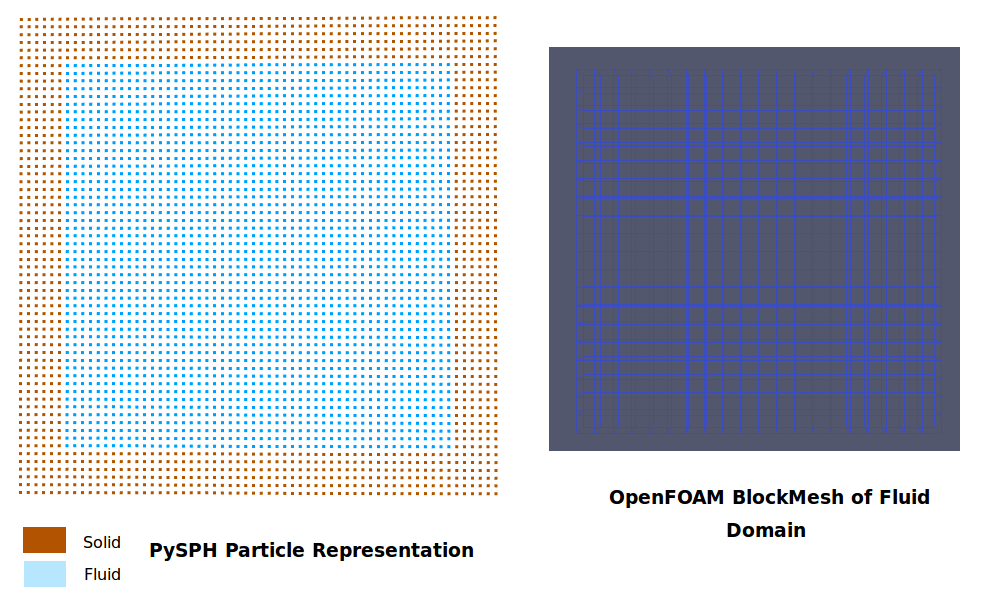
\includegraphics[scale = 0.25]{particle_rep.png}}
   \caption{Discretization in Meshfree and Grid Based Methods}
  \end{figure}
  \begin{itemize}\pause
   \item Particle Distribution can be completely arbitrary
   \item No explicit interconnectivity between particles
  \end{itemize}
 \end{frame}
 
 \begin{frame} %slide 5
  \frametitle{The SPH Method: Numerical Discretization}
  \begin{itemize}
  \item Consider a Scalar Field A(\textbf{r},\textit{t}), 
   \begin{eqnarray}
    A(\textbf{r},t)  = (A\ast \delta)(\textbf{r},t) \pause 
                     = \int_{\varOmega} A(\textbf{r'},t) \delta (\textbf{r - r'}) d^{3}\textbf{r'} \nonumber
   \end{eqnarray} \pause
  \item This $\delta$ is approached through an Interpolation Kernel \\ \textit{w$_h$}(\textbf{r - r'}). \pause 
  \item Kernel/Continuous Approximation of A is,
   \begin{eqnarray}
    A(\textbf{r},t) \approx [A]_{c}(\textbf{r},t)= \int_{\varOmega} A(\textbf{r'},t) \textit{w$_h$(\textbf{r - r'})} d^{3}\textbf{r'} \nonumber
   \end{eqnarray} \pause
   \item The Kernel is a Real function and has non-zero values on a compact/infinite sized support
   \item The support depends on the \textbf{Smoothing Length}, \textit{h}.
  \end{itemize}
 \end{frame}
% 
 \begin{frame} %slide 6
  \frametitle{The SPH Method: Numerical Discretization}
  %\setstcolor{red}
  \begin{itemize}
   \item Kernel Properties (for $[A]_{c}$ to be First Order Accurate)
   \begin{itemize}
    \item It's integral over the domain should be 1
    \item It's first moment should be 0; \pause satisfied by taking a symmetrical Kernel
   \end{itemize} \pause
   \item Particle Approximation of A: $[A]_{c}$ approximated by a Riemann Sum
    \begin{eqnarray}
     [A]_{c}(\textbf{r},t) = \int_{\varOmega} A(\textbf{r'},t) \textit{w$_h$(\textbf{r - r'})} d^{3}\textbf{r'} \nonumber \\
     \approx \sum_{b}A(\textbf{$\bf{r}_b$},t)~\textit{w$_h$}(\textbf{$|\bf{r}-\bf{r}_b |$}) ~ \textit{V$_b$}\pause = [A]_{d} \nonumber \\ \pause
     \therefore [A]_{d} = \sum_{b}A(\textbf{$\bf{r}_b$},t)~\textit{w$_h$}(\textbf{$|\bf{r}_{ab} |$}) ~ \textit{V$_b$} ,\nonumber \\ 
     \forall a \in  \varOmega , \textbf{r}_{ab} = \textbf{r}_{a} - \textbf{r}_{b}  \nonumber
   \end{eqnarray}
 \end{itemize}
 \end{frame}
%  
 \begin{frame} %slide 7
  \frametitle{The SPH Method}
  \begin{itemize}
   \item The properties of each particle {\bf{`a'}} depends on the {\bf{`b'}} particles in its neighbourhood defined by the Smoothing Length {\bf{`h'}} \pause
   \item A Nearest Neighbour Particle Search (NNPS) algorithm takes care of which particles {\bf{`b'}} influence the properties of {\bf{`a'}} \pause
   \begin{itemize}
    \item pySPH implements a Linked List NNPS algorithm by default\pause
   \end{itemize}
   \item The Finite Element Method and SPH
   \begin{itemize}
    \item Both Methods represent the field variables as linear combinations of basis functions \pause
    \item FEM constructs these basis functions from the grid and SPH constructs them based on the kernel \pause
    \item The FEM basis functions are stationary, while those of SPH move along with the particles.\\
    i.e. if {\bf{`B'}} are the SPH Basis functions then $\frac{D{\bf{B}}}{Dt} = 0$ 
   \end{itemize}
  \end{itemize}
 \end{frame}

 \begin{frame} %slide 8
  \frametitle{The Discrete Element Method}
  \begin{itemize}
   \item It is a numerical scheme which allows finite rotations and displacements of discrete bodies
   \item The bodies interact with their nearest neighbours through Contact Laws; the interactions create new or destroy earlier contacts.
   \item {\bf{Soft Contact}} Method
   \begin{itemize}
    \item The bodies are allowed to ``overlap''
    \item The amount and rate of the overlap gives incremental contact forces
    \item These contact forces are applied to Newton's laws to obtain new out of balance forces and moments
    \item From the forces and moments, the velocities and displacements are evaluated
   \end{itemize}
  \end{itemize}
 \end{frame}

 \begin{frame} %slide 9
 \frametitle{DEM and pySPH}
 \begin{itemize}
  \item DEM terminology:
  \begin{itemize}
   \item Contact Search: The procedure of keeping track of the bodies that are in contact with a given body in a time-step
   \item Boxing: Time saving mechanism wherein the working area is divided into squares/cubes (for 2D or 3D)
  \end{itemize}
  \item Calculation of Contact Force
  \begin{itemize}
   \item Ascertain if contact is present
   \item Calculate the amount of overlap
   \item Use the overlap in the contact model and compute the contact force
  \end{itemize}
  \item Since the bodies are represented as collections of particles in pySPH, explicit Boxing and Contact Search is not needed
  \item the NNPS keeps track of all those elements which are in contact and the smoothing length effectively computes the amount of overlap  
 \end{itemize}
 \end{frame}
%
 \begin{frame} %slide 10
  \frametitle{RigidBodyCollision Model}
  \begin{itemize}
  \item Models the 	contacts as a Spring and Dashpot system \pause
  \item Current PoC model implementation
  
   ~~Repulsive Force, ~~$f_{i,s} = -k(d-|{\bf{r_{ij}}}|)\frac{{\bf{r_{ij}}}}{|{\bf{r_{ij}}}|}$ \\
    ~~Damping Force, ~~$f_{i,d} = \eta ~ {\bf{v_{ij}}}$ \\ 
    ~~Shear Force, ~~ $f_{i,t} = k_{t} ~ {\bf{v_{ij,{\it{t}}}}}$\\
    ~~~~where, \\
    ~~~~~~{\it{k}} $=$ Spring Coefficient, \\
    ~~~~~~{\it{k$_t$}} $=$ Coefficient of Shear, \\
    ~~~~~~$\eta =$ Damping Coefficient,\\
    ~~~~~~d $=$ diameter of elements comprising the body\\ 
    ~~~~~~${\bf{r_{ij}}} = \textbf{r}_{i} - \textbf{r}_{j}$,\\
    ~~~~~~${\bf{v_{ij}}} =\textbf{v}_{i} - \textbf{v}_{j} $ \\
    ~~~~~~Relative Tangential Velocity, $${\bf{v_{ij,{\it{t}}}}} = {\bf{v_{ij}}} - \left({\bf{v_{ij}}} \cdot \frac{{\bf{r_{ij}}}}{|{\bf{r_{ij}}}|}\right) \frac{{\bf{r_{ij}}}}{|{\bf{r_{ij}}}|} $$\\
  \end{itemize}
 \end{frame}
%
 \begin{frame} %slide 11
  \frametitle{RigidBodyCollision Model}
  \begin{itemize}
   \item Total Contact Force, $$F_c = \sum_{i\in RigidBody} \left(f_{i,s} + f_{i,d} + f_{i,t} \right)$$
   \item Total Torque due to contact, $$T_C = \sum_{i\in RigidBody} \left[ r_{i} \times \left(f_{i,s} + f_{i,d} + f_{i,t} \right)\right] $$
  \end{itemize}
 \end{frame}
 
%  \begin{frame} % slide 12
%  \frametitle{Prospective Projects}
%  	\textbf{2. An Object Oriented Design for 3D Boundary Collisions}
%  	\begin{itemize}
%  		\item Work suggested by Dr. Prabhu Ramachandran \pause 
%  		\item Roadblocks in the DSMC and pySPH front \pause
%  		\begin{itemize}
%  		 \item Unavoidable Commitments for Prof. Ramachandran
%  		 \item Absolute zero functionality of the pySPH framework in terms of DSMC
%  		 \item Constraints of working remotely and communicating effectively
%  		\end{itemize}\pause
%  		\item Project Description:\\ To develop a mechanism by which particle collisions with boundary surfaces can be detected. Also develop a mechanism to estimate the position of the particle after collision. \pause
%  		\item Project Outcomes:
%  		 \begin{itemize}
%  		  \item pySPH will have capability to simulate particle collisions within objects of arbitrary shapes.
%  		  \item Work with test driven software development. 
%  		 \end{itemize} \pause
%  		 \item Software Tools : Python and pySPH
%  	\end{itemize}
% \end{frame}
%
%  \begin{frame} % slide 13
%  \frametitle{Ending Thoughts}
%  	\begin{itemize}
%  	 \item Worst Case Scenario \pause
%  	  \begin{itemize}
%  	  	\item Continue with 3D Boundary Collisions Problem
%  	 	\item Shift to an Incompressible Flow Problem to solve using SPH in pySPH \pause
%  	  \end{itemize}
%  	 \item Best Case Scenario \pause
%  	  \begin{itemize}
%  	  	\item Work on the Gas Turbine and Rocket Engine Combustor problem in IITB \\\pause
%  		      Work on DSMC and pySPH in my spare time ( not as part of the MTech Project )  
%  	  \end{itemize}
%    \end{itemize}
%  \end{frame}

 \begin{frame} %slide 14
  \frametitle{Thank you!}

  \begin{center}
    \large{Questions?}   
  \end{center}    
  
 \end{frame}


\end{document}
